%%==================================================================%%
%% Author : Abascal Fern�ndez, Patricia                             %%
%% Author : S�nchez Barreiro, Pablo                                 %%
%% Version: 1.2, 15/05/2013                                         %%
%%                                                                  %%
%% Memoria del Proyecto Fin de Carrera                              %%
%% Application Engineering/Generadores de C�digo C#                 %%
%%==================================================================%%
Tras explicar en detalle el algoritmo necesario para obtener las versiones clean de las clases y m�todos en la secci�n \ref{app:sec:alg}, se procede a comentar la implementaci�n de los generadores de c�digo correspondientes. La figura \ref{app:fig:templates} muestra la jerarqu�a de los generadores de c�digo implementados.

\begin{figure}[!tb]
  \center
  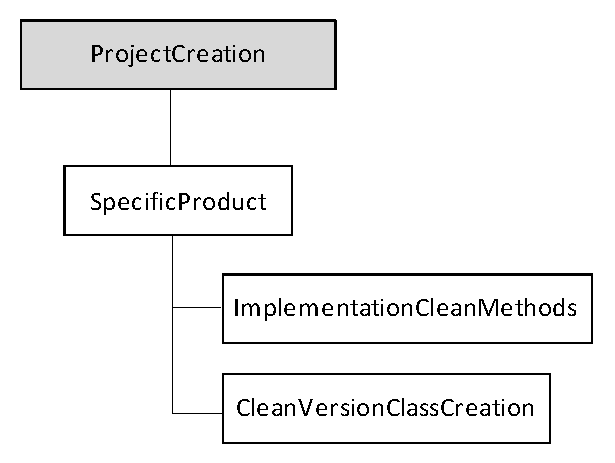
\includegraphics[scale=0.60,angle=0]{applicationEngineering/images/TemplatesAppEngineering.eps} \\
  \caption{Jerarqu�a de los generadores de c�digo implementados en la fase de Ingenier�a de Aplicaci�n}
  \label{app:fig:templates}
\end{figure}

El punto de partida es id�ntico al utilizado para la fase de \emph{Ingenier�a del Dominio}; es decir, el generador de c�digo llamado \imp{ProjectCreation}, a partir del cual se invoca a la plantilla \imp{SpecificProduct} que genera los ficheros fuente correspondientes a la implementaci�n del caso concreto determinado por el profile del modelo. Para ello se hacen llamadas a las plantillas descritas en forma de �rbol en la figura \ref{app:fig:templates}. Se procede a explicar brevemente el funcionamiento de cada una de ellas:  
 \begin{itemize}
   \item MergeClasses, genera un listado de los paquetes del modelo y los paquetes directamente relacionados con los mismos.
   \item SpecificPath, genera un conjunto que incluye aquellos paquetes que necesitan ser implementado para el camino espec�fico seleccionado.
   \item ExtractClassesAndOperations, genera un listado con cada paquete, por el camino espec�fico, y sus correspondientes clases y versiones clean de las operaciones que implementa.
   \item FuseElements, fusiona las operaciones de las clases, con el mismo nombre, que est�n en paquetes diferentes.
   \item ImplementationCleanMethods, genera la implementaci�n final de los m�todos clean (con sus correspondientes implementaciones internas).
   \item BranchFromSpecificProduct, extrae las versiones m�s profundas de cada m�todo en una rama concreta.
   \item IsThereMethod, indica si un m�todo est� implementado en el paquete dado.
   \item RearrangeMethods, selecciona de todas las ramas del proyecto espec�fico aquellas versiones de los m�todos m�s profundas y elimina las redundancias mediante el an�lisis de la alcanzabilidad.
   \item SpecificMethods, genera la implementaci�n para la versi�n clean de cada clase y la implementaci�n interna de sus m�todos.
   \item InternParams, genera los par�metros para las llamadas internas de los m�todos.
   \item CleanVersionClassCreation, una vez creados los elementos a generar, esta plantilla genera la estructura completa del fichero resultante.
   \item SpecificProductOperations, implementa funciones de uso recurrente a lo largo del resto de plantillas para simplificar el proceso. Entre las funciones implementadas est� la accesibilidad entre dos paquetes o la generaci�n de los paquetes para el caso espec�fico a analizar.
 \end{itemize}

Una vez explicado el funcionamiento de los generadores de c�digo, en la siguiente secci�n se proceder� a explicar la fase de pruebas de esta etapa del proyecto.
